\subsection{Full NLO QCD corrections and matching to parton showers}
\label{sec:fullPS}

%\textit{Authors:} S. Borowka, N. Greiner, G. Heinrich, S.P. Jones, M. Kerner, J. Schlenk, U. Schubert, T. Zirke (1604.06447+1608.04798)

\textbf{Sophia Borowka, Nicolas Greiner, Gudrun Heinrich, Stephen P. Jones, Matthias Kerner, Johannes Schlenk, Ulrich Schubert, Tom Zirke}~\cite{Borowka:2016ehy,Borowka:2016ypz,Heinrich:2017kxx,Jones:2017giv,Heinrich:2019bkc}.

\noindent In this section we briefly describe the calculation of the NLO QCD corrections to $gg\to hh$ including the full top quark mass dependence via a numerical method based on sector decomposition~\cite{Binoth:2000ps,Borowka:2015mxa}, explained in detail in Refs.~\cite{Borowka:2016ehy,Borowka:2016ypz}, and the matching of these fixed-order results to parton showers~\cite{Heinrich:2017kxx,Jones:2017giv,Heinrich:2019bkc}.

\subsubsection{Method}
\label{intro_ampli}

%%As already mentioned in section~\ref{sec:hhew},
%The amplitude can be decomposed into form factors as
%\begin{align}
%&{\cal M}_{ab}=\delta_{ab}\,\epsilon^\mu (p_1,n_1)\epsilon^\nu (p_2,n_2)\,{\cal
%  M}_{\mu\nu}\label{eq:FFdeco}\\
%&{\cal M}^{\mu\nu}=\frac{\alpha_s}{8\pi v^2}\left(F_1(\hat{s},\hat{t},m_h^2,m_t^2,D)\;T_1 ^{\mu\nu}+F_2(\hat{s},\hat{t},m_h^2,m_t^2,D)\;T_2 ^{\mu\nu}\right)\;,\nonumber
%\end{align}
%where $D$ denotes the space-time dimension.
%The form factors are related to helicity amplitudes by
% \begin{align}
%{\cal M}^{++}&={\cal M}^{--}=-\frac{\alpha_s}{8\pi v^2} \,F_1\nonumber\\
%{\cal M}^{+-}&={\cal M}^{-+}=-\frac{\alpha_s}{8\pi v^2} \,F_2\;.
%\end{align}
%We performed a projection onto form factors via appropriate projectors $P_{1,2}^{\mu\nu}$
%\begin{eqnarray*}
%P_1^{\mu\nu} {\cal M}_{\mu\nu}&=&\frac{\alpha_s}{8\pi v^2}\,F_1(\hat{s},\hat{t},m_h^2,m_t^2,D)\;, \\
%P_2^{\mu\nu} {\cal M}_{\mu\nu}&=&\frac{\alpha_s}{8\pi v^2}\,F_2(\hat{s},\hat{t},m_h^2,m_t^2,D)\;.
%\end{eqnarray*}
The virtual two-loop amplitude has been generated with an extension of the program \texttt{GoSam}~\cite{GoSam:2014yla,Braun:2025afl}, and the form factors extracted according to Eq.~\eqref{eq:in:ffe}.
The reduction of the integrals occurring in the amplitude to master integrals has been performed using \texttt{Reduze}~\cite{vonManteuffel:2012np}.
 A complete reduction had been achieved only for the planar sectors, while a partial reduction of the
non-planar sectors was sufficient for the numerical evaluation. This led to 145 planar master
integrals plus 70 non-planar integrals, and a further 112 integrals that differ by a crossing.
As these integrals contain four independent mass scales,
$\hat{s},\hat{t},m_t^2, m_h^2$, their analytical calculation is a hard task.
We calculated all integrals numerically using the program \texttt{SecDec}-3.0~\cite{Borowka:2015mxa}, which has since evolved into \texttt{pySecDec}~\cite{Borowka:2017idc,Heinrich:2023til}, using $\sim$16 dual \texttt{Nvidia Tesla K20X} GPU nodes.
%For the integration we used a quasi-Monte Carlo method based on a rank-one lattice rule~\cite{Li:2015foa,QMCActaNumerica,nuyens2006fast}.

The amplitudes for the real radiation have been generated with \texttt{GoSam}~\cite{GoSam:2014yla,Braun:2025afl}.
As the process is loop-induced, the NLO real corrections involve one-loop $2\to 3$ amplitudes where single-unresolved radiation can occur.
We used the Catani-Seymour dipole formalism~\cite{Catani:1996vz} to isolate the corresponding infrared poles.

The dependence on the trilinear Higgs boson self-coupling modifier
$\kappa_\lambda \equiv \lambda_{hhh}/\lambda_{hhh}^{\rm SM}$
was also assessed in Ref.~\cite{Borowka:2016ypz}, for the first time
at full NLO.
In the HTL at leading order, the $\kappa_\lambda$-dependence is
given by
\begin{align}
|{\cal M}|^2&\sim  \frac{2}{9} -  \frac{4}{3}\,m_h^2\,\frac{\kappa_\lambda}{\hat{s}-m_h^2} +
  2\,m_h^4\,\frac{\kappa_\lambda^2}{(\hat{s}-m_h^2)^2}\;.\label{eq:loheft}
\end{align}
For $\kappa_\lambda=1$, this expression vanishes at the Higgs boson pair production threshold
$\hat{s} \sim 4 m_h^2$. For larger values of $\kappa_\lambda$, the minimum is
shifted; the expression above has a double zero at
$\hat{s}=m_h^2(1+3\kappa_\lambda)$ due to the destructive interference between box- and
triangle-type contributions.
In the full theory, the amplitude does not vanish completely at these points,
but nonetheless also gets small.

\subsubsection{Results}
The total cross section at full NLO, at $\sqrt{s}=14$\,TeV, was found to be smaller than the Born-rescaled NLO cross section in the HTL by about 15\%, and smaller than the $\mathrm{NLO}_{\mathrm{FTapprox}}$ result by about 4\%.

Differential results for the Higgs boson pair invariant mass distribution $m_{hh}$ and the transverse momentum distribution of a Higgs boson, $p_{T,h}$, are shown in Fig.~\ref{fig:mhh}.
Comparing the full NLO result with the HTL prediction (called HEFT in Fig.~\ref{fig:mhh}), one can clearly see that the high-energy region is not well described by this approximation, even if it is rescaled with the full Born (called ``Born-improved HEFT'', blue curve). Without rescaling by the full Born (called ``basic HEFT''), the prediction fails to describe the distribution except in the very low-$m_{hh}$ bins, as this approximation is only valid below the production threshold of a virtual top quark pair. The dark green curve denotes the so-called $\mathrm{NLO}_{\mathrm{FTapprox}}$ (``approximate Full Theory'')~\cite{Maltoni:2014eza}, where the real radiation part is calculated with full $m_t$ dependence, while the virtual corrections are calculated in the HTL. This approximation has been lifted to NNLO accuracy in Ref.~\cite{Grazzini:2018bsd}, described in Section~\ref{sec:NNLO_FTapprox}.


\begin{figure}
\centering
\begin{subfigure}{0.49\textwidth}
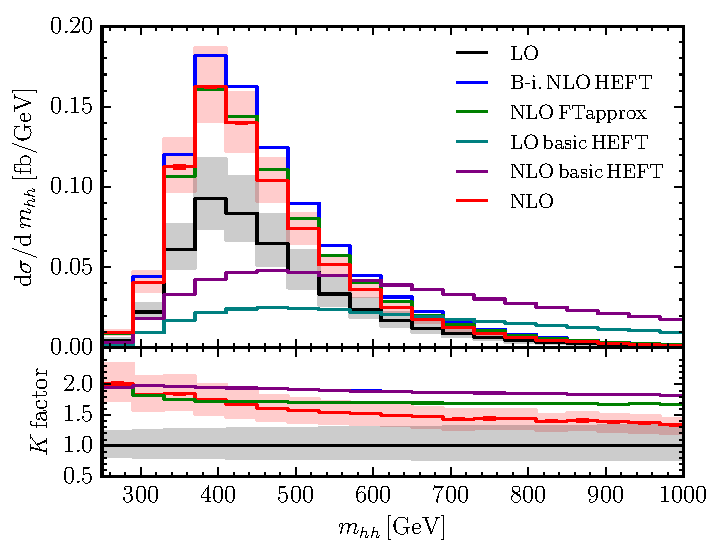
\includegraphics[width=\textwidth]{NLO_QCD_SM/NLOmtPS/Images/mhh_Kfac_14TeV_lambda1}
\caption{Higgs boson pair invariant mass distribution.\label{subfig:mhh}}
\end{subfigure}
\begin{subfigure}{0.49\textwidth}
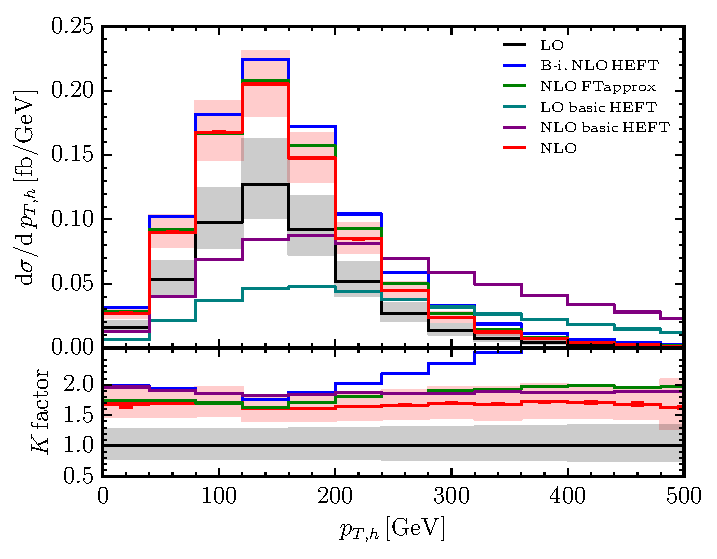
\includegraphics[width=\textwidth]{NLO_QCD_SM/NLOmtPS/Images/pth_Kfac_14TeV_lambda1}
\caption{$p_{T,h}$ distribution.\label{subfig:pth14}}
\end{subfigure}
\caption{(a) Higgs boson pair invariant mass distribution $m_{hh}$, (b) transverse momentum distribution of (any) Higgs boson, $p_{T,h}$, both at
  $\sqrt{s}=14$\,TeV. In this figure, HEFT denotes the HTL, and ``basic'' means not rescaled by the full-$m_t$ Born amplitude. Figures from Ref.~\cite{Borowka:2016ypz}.\label{fig:mhh}}
\end{figure}

\subsubsection{Matching to parton showers}

The NLO result calculated in
Refs.~\cite{Borowka:2016ehy,Borowka:2016ypz} has been matched to the {\tt Powheg-Box-V2}~\cite{Alioli:2010xd} and {\tt MG5\_aMC@NLO}~\cite{Alwall:2014hca} in Ref.~\cite{Heinrich:2017kxx} and to {\tt Sherpa}~\cite{Gleisberg:2008ta} in Ref.~\cite{Jones:2017giv}, where the {\tt Powheg-Box-V2} implementation, i.e. the public code {\tt ggHH}, was later extended to include variations of the trilinear Higgs boson self-coupling~\cite{Heinrich:2019bkc} and the leading five anomalous couplings within non-linear Higgs Effective Field Theory (HEFT)~\cite{Buchalla:2018yce,Heinrich:2020ckp}.
In Refs.~\cite{Heinrich:2017kxx,Heinrich:2020ckp} it has been demonstrated that the differences between different parton showers and matching schemes can be quite large for radiation-sensitive observables such as the net transverse momentum of the Higgs boson pair, while they are very moderate for the invariant mass of the Higgs boson pair, see Fig.~\ref{fig:gghh_nlo_shower}.
It also has been shown that the NLO results in the HTL can differ more from the full NLO result than some prominent EFT benchmark points, underlining again the importance of the NLO corrections with full top quark mass dependence.

The code {\tt ggHH\_SMEFT} contains NLO QCD results combined with leading and subleading operators in SMEFT~\cite{Heinrich:2022idm,Heinrich:2023rsd}, as well as running Wilson coefficients~\cite{Heinrich:2024rtg}, see also Ref.~\cite{Alasfar:2023xpc} for Effective Field Theory descriptions of Higgs boson pair production. This code can be interfaced to parton showers within the {\tt Powheg-Box-V2} in the same way as the {\tt ggHH} code.

\begin{figure}
\centering
\begin{subfigure}{0.49\textwidth}
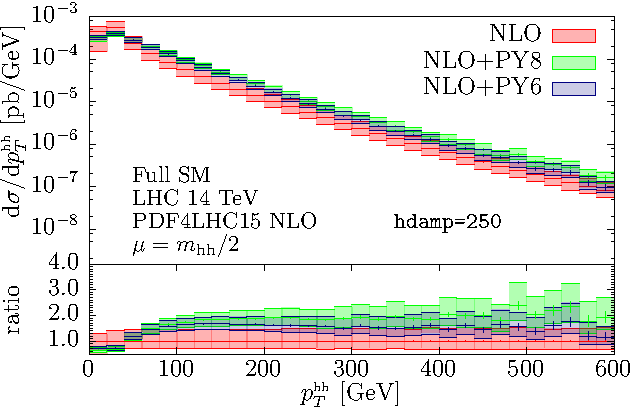
\includegraphics[width=\textwidth]{NLO_QCD_SM/NLOmtPS/Images/NLO_SWR_hdamp_ptHH_full_py6}
\caption{Figure from Ref.~\cite{Heinrich:2017kxx}.\label{subfig:pthh_pythia_shower}}
\end{subfigure}
\begin{subfigure}{0.49\textwidth}
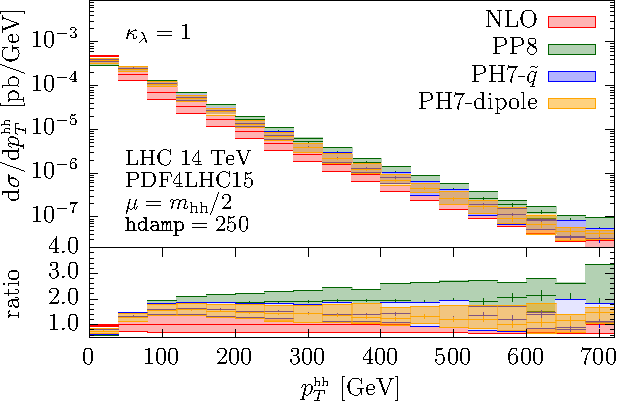
\includegraphics[width=\textwidth]{NLO_QCD_SM/NLOmtPS/Images/NLO_PP8_PH7_PH7D_cHHH_1_ptHH}
\caption{Figure from Ref.~\cite{Heinrich:2019bkc}.\label{subfig:pthh_herwig_shower}}
\end{subfigure}
\caption{Higgs boson pair transverse momentum spectrum, comparing fixed-order NLO with different parton showers. All results are based on the {\tt ggHH} ({\tt Powheg-Box-V2}) code. (a) Comparison of fixed-order NLO with its matching to Pythia6 (PY6) and \texttt{Pythia 8} (PY8)~\cite{Sjostrand:2014zea}; (b) comparison of \texttt{Pythia 8} (PY8) with the \texttt{Herwig 7}~\cite{Bellm:2017bvx,Bellm:2025pcw} $\tilde{q}$ and dipole showers, respectively.\label{fig:gghh_nlo_shower}}
\end{figure}
